\section{Durchführung}
Zunächst müssen die Apparatekonstanten, die Winkelrichtgröße $D$ und das Trägheitsmoment
der Drillachse $I_D$, bestimmt werden. Für die Winkelrichtgröße wird auf der Apparatur
eine nahezu Masselose Stange angebracht und die Kraft bei verschiedenen Auslenkungen
mithilfe einer Federwaage gemessen. Dabei ist wichtig, dass die Federwaage senkrecht gehalten wird.
Für das Trägheitsmoment der Drillachse werden an der Stange nun zwei identische Massen mit
gleichen Abständen zur Drehachse angebracht. Nun wird die Schwingungsdauer des Systems
bei verschiedenen Abständen der Massen zur Drehachse gemessen.
Die bestimmten Apparatekonstanten müssen bei den Rechnungen berücksichtigt weden.

Daraufhin können nun die Trägheitsmomente verschiedener Körper über die Schwingungsdauer
bestimmt werden. In diesem Fall einer Kugel, eines Zylinders und einer Puppe in
zwei verschiedenen Stellungen. Dafür werden die verschiedenen geometrischen Körper
auf der Apparatur angebracht, mit dem Schwerpunkt auf der Drehachse. Nun werden die Körper
aus ihrer Ausgangsposition ausgelenkt und die Schwingungsdauer wird gemessen.

Die Stellungen der Puppe sind in Abbildung (\ref{fig:Abb3}) schematisch dargestellt. In unserem Fall
sind bei der linken Position auf der Abbildung die Arme nach oben gestreckt und nicht nach unten.

\begin{figure}
  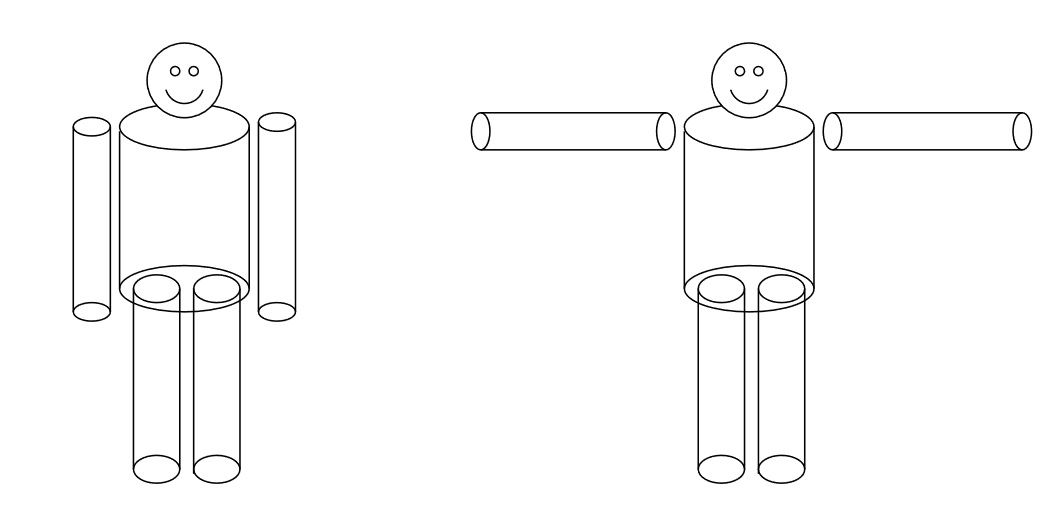
\includegraphics[width=\textwidth]{Bild3.jpg}
  \caption{Vereinfachte Darstellung der Modelpuppe [1].}
  \label{fig:Abb3}
\end{figure}
